\documentclass[a4paper,10pt]{scrartcl}
% \usepackage[latin1]{inputenc}
\usepackage[utf8]{inputenc}
\usepackage[ngerman]{babel}
\usepackage{url}
\usepackage{graphicx}
\usepackage{geometry}
\usepackage{graphicx}
\usepackage{amssymb}
\usepackage{marvosym}
\usepackage{amsmath}
\usepackage{lscape}
\usepackage{array}
\usepackage{listings}
\usepackage{color}
\usepackage{wasysym}
\usepackage{hyperref}
\usepackage{fancyvrb}
\bibliographystyle{plain}

\newcolumntype{L}[1]{>{\raggedright\arraybackslash}p{#1}} % linksbündig mit Breitenangabe
\newcolumntype{C}[1]{>{\centering\arraybackslash}p{#1}} % zentriert mit Breitenangabe
\newcolumntype{R}[1]{>{\raggedleft\arraybackslash}p{#1}} % rechtsbündig mit Breitenangabe

\geometry{verbose,tmargin=2.5cm,bmargin=2.5cm,lmargin=2.5cm,rmargin=3.5cm,headheight=80pt}

% Title Page
\subject{Algorithmen für geografische Informationssysteme}
\title{Projekt Viewshed Analysis}
\author{Moritz Beck, Bernhard Häussner, \\ Christina Hempfling, Jona Kalkus}
\date{29. Juli 2015}

\begin{document}
\maketitle

\section{Einleitung}
In unserem Projekt zur Vorlesung ``Algorithmen für geografische Informationssysteme'' stellen wir das Problem der ``Viewshed''-Analyse vor und 
vergleichen verschiedene Lösungs-Algorithmen. \\ Der englische Begriff \textit{viewshed} ist definiert als \textit{die geografische Fläche, die 
von einem bestimmtem Standpunkt aus sichtbar ist}. Der viewshed wird beispielweise bei folgenden Problemstellungen benötigt:
\begin{itemize}
 \item Bestimmung günstiger Standorte für Sendemasten
 \item Finden von Aussichtspunkten (z.B. im Gebirge), um Wanderwege planen zu können
 \item Finden von versteckten Punkten (z.B. für militärische Zwecke)
 \item Finden von besonders schönen Routen, z.B. entlang der Küste 
\end{itemize}
\begin{figure}[!ht]
\begin{minipage}{0.45\textwidth}
\centering
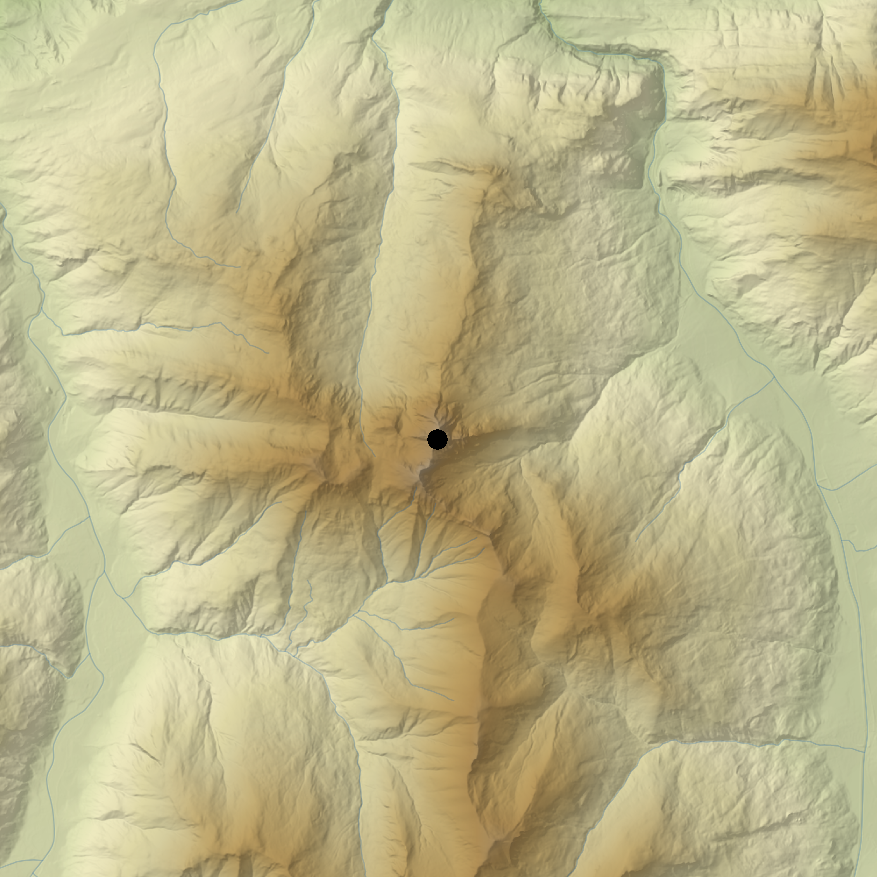
\includegraphics[scale=0.85]{bilder/berg_viewpoint}
\caption{Landkarte im Gebirge, der Standpunkt ist schwarz markiert}
\end{minipage}
\hfill
\begin{minipage}{0.45\textwidth}
\centering
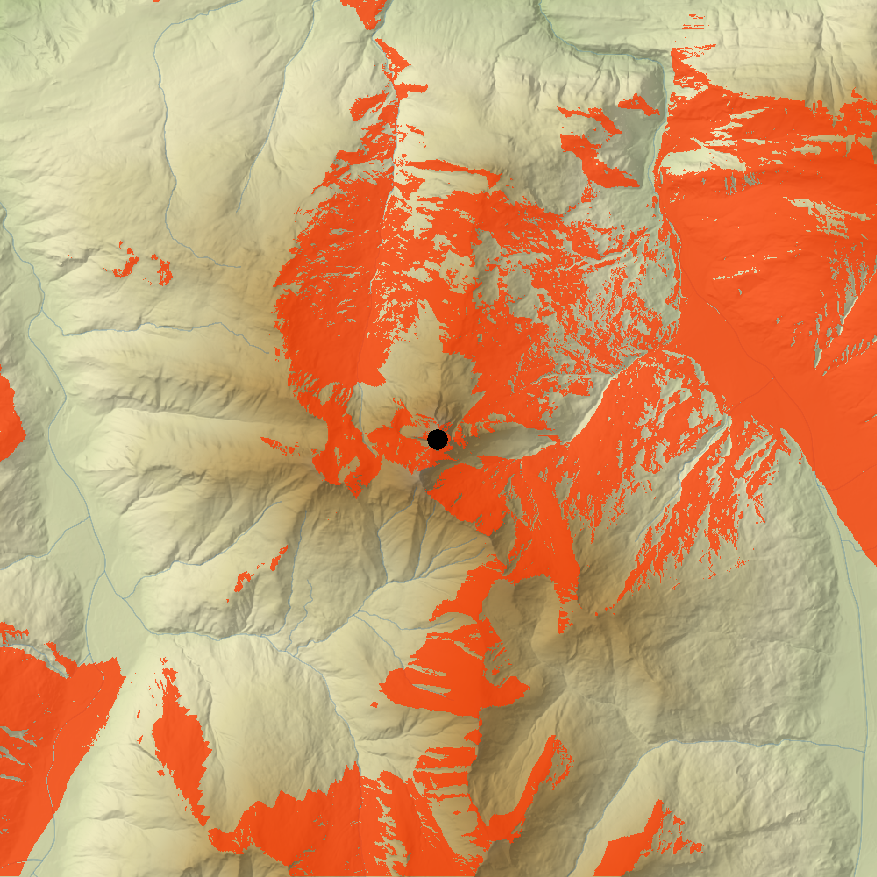
\includegraphics[scale=0.85]{bilder/berg_viewshed}
\caption{Die rote Fläche zeigt den vom Standpunkt aus sichtbaren Teil des Gebiets}
\end{minipage}
\end{figure}

Um den viewshed bestimmen zu können, ist ein sogenanntes \textit{digital elevation model} (DEM) nötig. 
Dieses digitale Höhenmodell ist eine Rasterkarte und enthält die Höhendaten des zugrunde liegenden Gebietes. 
Dargestellt wird das DEM als zweidimensionales Array, in dem die Höhendaten gespeichert sind. 

\noindent Für die Berechnung des viewsheds wird neben dem Höhenmodell auch ein Standpunkt benötigt, von welchem ausgehend die Sichtbarkeit anderer Punkte bestimmt werden soll. 
Sofern der Standpunkt oberhalb des Bodenniveaus liegen soll (etwa für Sendemasten, Einbeziehung der Augenhöhe oä.) kann zusätzlich eine Höhenangabe angegeben werden. 

%\noindent Ein DEM ist eine zwei- oder dreidimensionale Darstellung einer geografischen Karte und enthält die Höhendaten des dargestellten Gebiets. 
%Für unsere Problemstellung ist die zweidimensionale Variante ausreichend.

%\noindent In einem DEM, welches als zweidimensionales Array dargestellt werden kann, wird ein Punkt als Standort gewählt. Um z.B. die Höhe eines 
%Sendemasten miteinzuberechnen, kann auch eine zusätzliche Höhe angegeben werden, welche auf die Höhe des Standorts addiert wird.

\noindent Als Testdaten wurden DEMs der Bayerischen Vermessungsverwaltung \cite{berchtesgaden} und des Salzburger Geographischen Informationssystems 
\cite{salzburg} verwendet. Da die Testdaten in einer simplen Textdatei im ASCII-Grid Format (siehe Abbildung \ref{testfile}) zur Verfügung gestellt werden, lassen sich die Daten leicht auslesen und weiterverarbeiten.

\begin{figure}[!ht]
 \centering
 \begin{BVerbatim}
ncols         501
nrows         1001
xllcorner     4490660
yllcorner     5320200
cellsize      2
558.21 558.13 558.08 557.99 557.93 557.81 557.7  ....
558.1 558.06 557.95 557.89 557.83 557.73 557.6 ....
557.91 557.85 557.78 557.75 557.67 557.58 557.47 ...
557.81 557.78 557.7 557.66 557.56 557.48 557.4  ...
557.64 557.6 557.54 557.46 557.44 557.36 557.23  ...
557.59 557.51 557.46 557.38 557.37 557.28 557.15 ...
...
\end{BVerbatim}
\caption{DEM-Datei mit Angabe der Breite (ncols) und Höhe (nrows) des DEMs sowie der Größe einer Zelle (hier: 2 Meter)}
\label{testfile}
\end{figure}

\noindent Als Programmiersprache wurde Java (Version 1.8) verwendet. Zur Visualisierung der Daten wurde QGIS verwendet. 


\newpage
\section{Der naive Algorithmus}
\newpage
\section{Der Algorithmus von van Kreveld}

Die Laufzeit des naiven Algorithmus in $O(n^3)$ liegt (wobei $n$ das Maximum aus Breite und Höhe des DEM ist), gibt es einige Überlegungen zu 
schnelleren Algorithmen. Als eine Art untere Schranke für die Laufzeit der viewshed-Berechnung kann das Einlesen des DEMs gesehen werden, welches 
in $O(n^2)$ liegt. Somit sollte eine Verbesserung der Laufzeit möglichst nahe an diese untere Schranke heranreichen. Im Paper von van Kreveld 
\cite{vanKrev} werden Optimierungsvorschläge vorgestellt und gezeigt, dass die Laufzeit auf $O(n^2)\log n$ verbessert werden kann. 

\subsection{Der sweep line-Algorithmus}
Van Krevelds Algorithmus beruht auf dem Prinzip der sogenannten ``sweep line''. Allgemein ist eine sweep line eine (horizontale) Linie, 
welche über eine Menge von Objekten in einer Ebene ``streicht'' und dabei alle relevanten Informationen bezüglich einer Problemstellung ausliest und 
sammelt, damit diese dann weiterverarbeitet werden können. Beispielsweise kann die Linie über eine Ebene streichen und dabei den Beginn und das Ende 
geometrischer Formen detektieren (siehe Abbildung \ref{sweep}). Da sich die Menge der Objekte, die die Linie schneiden, oft ändert, muss für das 
Sammeln der Informationen eine flexible Datenstruktur gewählt werden. Hierfür eignet sich ein balancierter binärer Baum, welcher als 
``Statusstruktur'' bezeichnet wird (siehe Abbildung \ref{stat}) und die Änderungen des Status festzuhalten. 

\begin{figure}[!ht]
\begin{minipage}{0.55\textwidth}
\centering
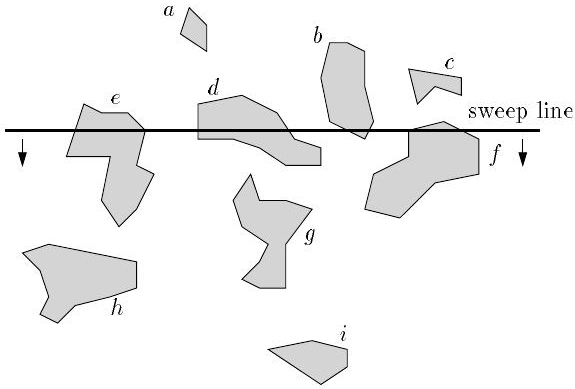
\includegraphics[scale=0.62]{bilder/sweep}
\caption{sweep line streicht über Objekte in einer Ebene}
\label{sweep}
\end{minipage}
\hfill
\begin{minipage}{0.4\textwidth}
\centering
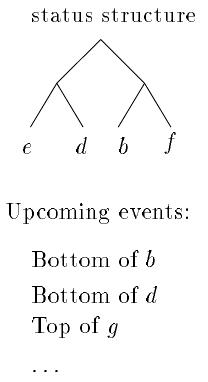
\includegraphics[scale=0.67]{bilder/statstruc}
\caption{Statusstruktur, in der die auftretenden Ereignisse gespeichert werden}
\label{stat}
\end{minipage}
\end{figure}

Um zu wissen, wann sich der Status ändert -- also wenn die Linie beispielsweise ein neues Objekt schneidet -- werden sogenannte ``events'' eingeführt
und ebenfalls in einer eigenen Datenstruktur gespeichert. Hierfür kann eine Prioritätswarteschlange oder ebenfalls ein balancierter binärer Baum 
benutzt werden. Für das Beispiel der viewshed-Analyse ist die Definition folgender events sinnvoll: 
\begin{itemize}
 \item die sweep line detektiert beim Streichen über das DEM einen neuen Pixel
 \item die sweep line detektiert beim Streichen über das DEM den Mittelpunkt eines Pixels
 \item die sweep line detektiert beim Streichen über das DEM die ``letzte Ecke'' eines Pixels, er wurde also von der Linie komplett durchlaufen
\end{itemize}

Der Pseudocode für den sweep line-Algorithmus ist in Abbildung \ref{pseudo} zu sehen.
\vspace{5pt}

Aufgrund der gewählten Datenstruktur eines balancierten binären Baums für die Statusstruktur erfolgt das Einfügen und Löschen von Daten sowie der 
Zugriff darauf in $O(\log n)$ Zeit, wodurch hier gegenüber dem naiven Algorithmus eine deutliche Verbesserung der Laufzeit erreicht wird. Das 
Einlesen des DEMs erfolgt weiterhin in $O(n^2)$ Zeit, doch durch das Benutzen des sweep line-Algorithmus kommt nun nur noch ein Anteil von 
$O(\log n)$ hinzu, was in einer Gesamtlaufzeit von $O(n^2\log n)$ resultiert.

\begin{figure}[!ht]
 \centering
 \begin{BVerbatim}
Initialisiere die event list und die Statusstruktur
 Solange die event list noch nicht leer ist 
  Do Nimm das erste Element aus der Liste 
     Wenn ein neues Objekt die sweep line schneidet
	       füge es in die Statusstruktur ein
     Wenn ein Objekt nicht länger von der sweep line geschnitten wird
	       lösche es aus der Statusstruktur heraus
     Falls möglich, führe die gewünschten Berechnungen mit Hilfe der Statusstruktur durch      
     Falls nötig, füge neue events in die event list ein
  EndDo
\end{BVerbatim}
\caption{Pseudocode für sweep line-Algorithmus}
\label{pseudo}
\end{figure}

\subsection{Anpassung des sweep line-Algorithmus für das Problem der viewshed-Analyse}
\label{sweep_adjust}
Um den sweep line-Algorithmus für die viewshed-Analyse benutzen zu können, müssen ein paar kleine Anpassungen vorgenommen werden. Im Gegensatz zu 
der in Abbildung \ref{sweep} gezeigten horizontalen sweep line, legt van Kreveld den Ursprung der Linie auf die Koordinaten des Standorts und lässt 
sie dann wie bei einem Radar in einer Kreisbewegung über das DEM streichen (siehe Abbildung \ref{sweep_k}).

\begin{figure}[!ht]
 \centering
 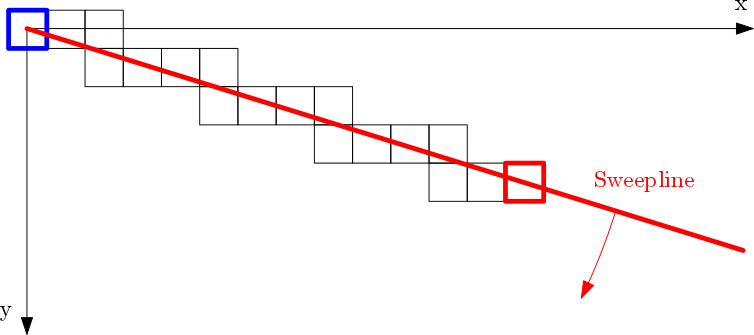
\includegraphics[scale=0.45]{bilder/sweep_kreveld}
 \caption{Definition der sweep line im Algorithmus von van Kreveld. Der Standort ist blau markiert, der rot umrandete Pixel ist ein Randpixel des 
 DEMs.}
 \label{sweep_k}
\end{figure}

In unserer Implementierung definieren wir den Winkel $0^\circ$ für die sweep line parallel zur x-Achse und sie schneidet zu Beginn des Algorithmus 
alle Pixel rechts neben dem Standort. Zudem lassen wir die Linie -- wie die Abbildung zeigt -- \textbf{im} Uhrzeigersinn über das DEM kreisen. Im 
Gegensatz zur ``normalen'' sweep line, ist hier die Länge der sweep line nicht konstant, sondern hängt vom Setzen des Standorts im DEM ab. 

Weiterhin haben wir drei Klassen von events definiert: 
\begin{itemize}
 \item \textit{EventType\_IN}: die sweep line detektiert den Beginn eines Pixels im DEM 
 \item \textit{EventType\_CENTER}: die sweep line streicht über die Mitte eines Pixels,
 \item \textit{EventType\_OUT}: die sweep line detektiert das Ende eines Pixels im DEM, also die letzte Ecke, die überstrichen wird
\end{itemize}

Für jeden Pixel im DEM wird der Winkel zum Standort berechnet, unter dem die drei jeweiligen Eventtypen auftreten. Dies ist nötig, da alle Eventtypen 
in der event list nach dem Winkel zum Standort sortiert werden. Somit wird das Prinzip der kreisförmigen Bewegung der sweep line realisiert, da die 
Pixel der Reihe nach mit aufsteigendem Winkel abgearbeitet werden. 

Die Berechnung, ob ein Pixel vom Standort aus sichtbar ist, erfolgt mit Hilfe der Statusstruktur, welche in Kapitel \ref{tree} genauer beschrieben 
ist.

Unsere (erste) Implementierung des van Kreveld-Algorithmus lässt sich folgendermaßen als Pseusocode darstellen:

\begin{figure}[!ht]
 \centering
 \begin{BVerbatim}
  Initialisiere die Statusstruktur 
  Fülle die event list, indem für jeden Pixel im DEM die drei entsprechenden Eventtypen 
    in die event list eingefügt werden  
  Solange die event list noch nicht leer ist 
    Do Nimm das erste event aus der Liste 
      Falls Typ == EventType.IN
	  füge Pixel in die Statusstruktur ein
      Falls Typ == EventType.OUT
	  lösche Pixel in der Statusstruktur 
      Falls Typ == EventType.CENTER
	  berechne die Sichtbarkeit des Pixels mit Hilfe der in der Statusstruktur 
	  gespeicherten Daten
    EndDo

 \end{BVerbatim}
 \caption{Pseudocode für van Kreveld-Algorithmus}
 \label{pseudo_krev}
\end{figure}

Nach der Implementierung dieses Codes zeigten bereits die ersten Testläufe, dass dieser Algorithmus trotz der angepriesenen Verbesserung der Laufzeit 
wesentlich länger zur Berechnung eines viewsheds benötigte, als der naive Algorithmus. Im folgenden Kapitel werden unter Punkt \ref{speicher} daher 
die von uns identifizierten Probleme des Codes dargestellt und Lösungsvorschläge unterbreitet. 


\newpage
\section{Probleme}

\subsection{Datenstruktur der Statusstruktur}
\label{tree}
Die von van Kreveld vorgeschlagene Datenstruktur eines balancierten binären Baums ist in dieser Form noch nicht in Java 1.8 vorhanden. Daher mussten 
wir diese selbst implementieren.
Van Kreveld schlägt einen balancierten Binärbaum vor, der nur in den Blattknoten Pixel abspeichert
und in jedem inneren Knoten $v$ die maximale Steigung aller Blätter des Teilbaums mit Wurzel $v$ speichert.
Java stellt zwar balancierte Binärbäume zur Verfügung, allerdings können diese weder augmentiert werden,
noch speichern diese ihre Elemente ausschließlich in den Blattknoten.
Deshalb haben wir die Statusstruktur basierend auf Code für einen Rot-Schwarz-Baum im Java Development Kit (TreeMap.java) implementiert.
Sie stellt einen Rot-Schwarz-Baum dar, der -- im Gegensatz zu van Krevelds Vorschlag -- in \emph{jedem} Knoten einen Pixeleintrag abspeichert
und jeden Knoten $v$ um dessen Steigung (slope) und die maximale Steigung (maxSlope) aller Nachfahrknoten augmentiert.
Bereitgestellt werden die Methoden \verb|insert(HeightedPoint pt)|, \verb|delete(HeightedPoint pt)| und \verb|isVisible(HeightedPoint pt)|,
die die Operationen implementieren, die bei den Ereignissen \verb|IN|, \verb|OUT| beziehungsweise \verb|CENTER| ausgeführt werden.
Innerhalb der Statusstruktur sind die Pixel nach ihrer Distanz zum Standpunkt georgnet.
Weil in der Statusstruktur genau die Pixel gehalten werden, die auf der Sichtlinie liegen, bedeutet dies,
dass alle Pixel, die die Sicht auf einen bestimmten verdecken können, links diesen Pixels in dem Baum liegen.
Die Methode \verb|isVisible(HeightedPoint pt)| muss also nur logaritmisch viele Vergleiche durchführen, siehe Abbildung~\ref{fig:isVisible}.

\begin{figure}[ht]
    \centering
    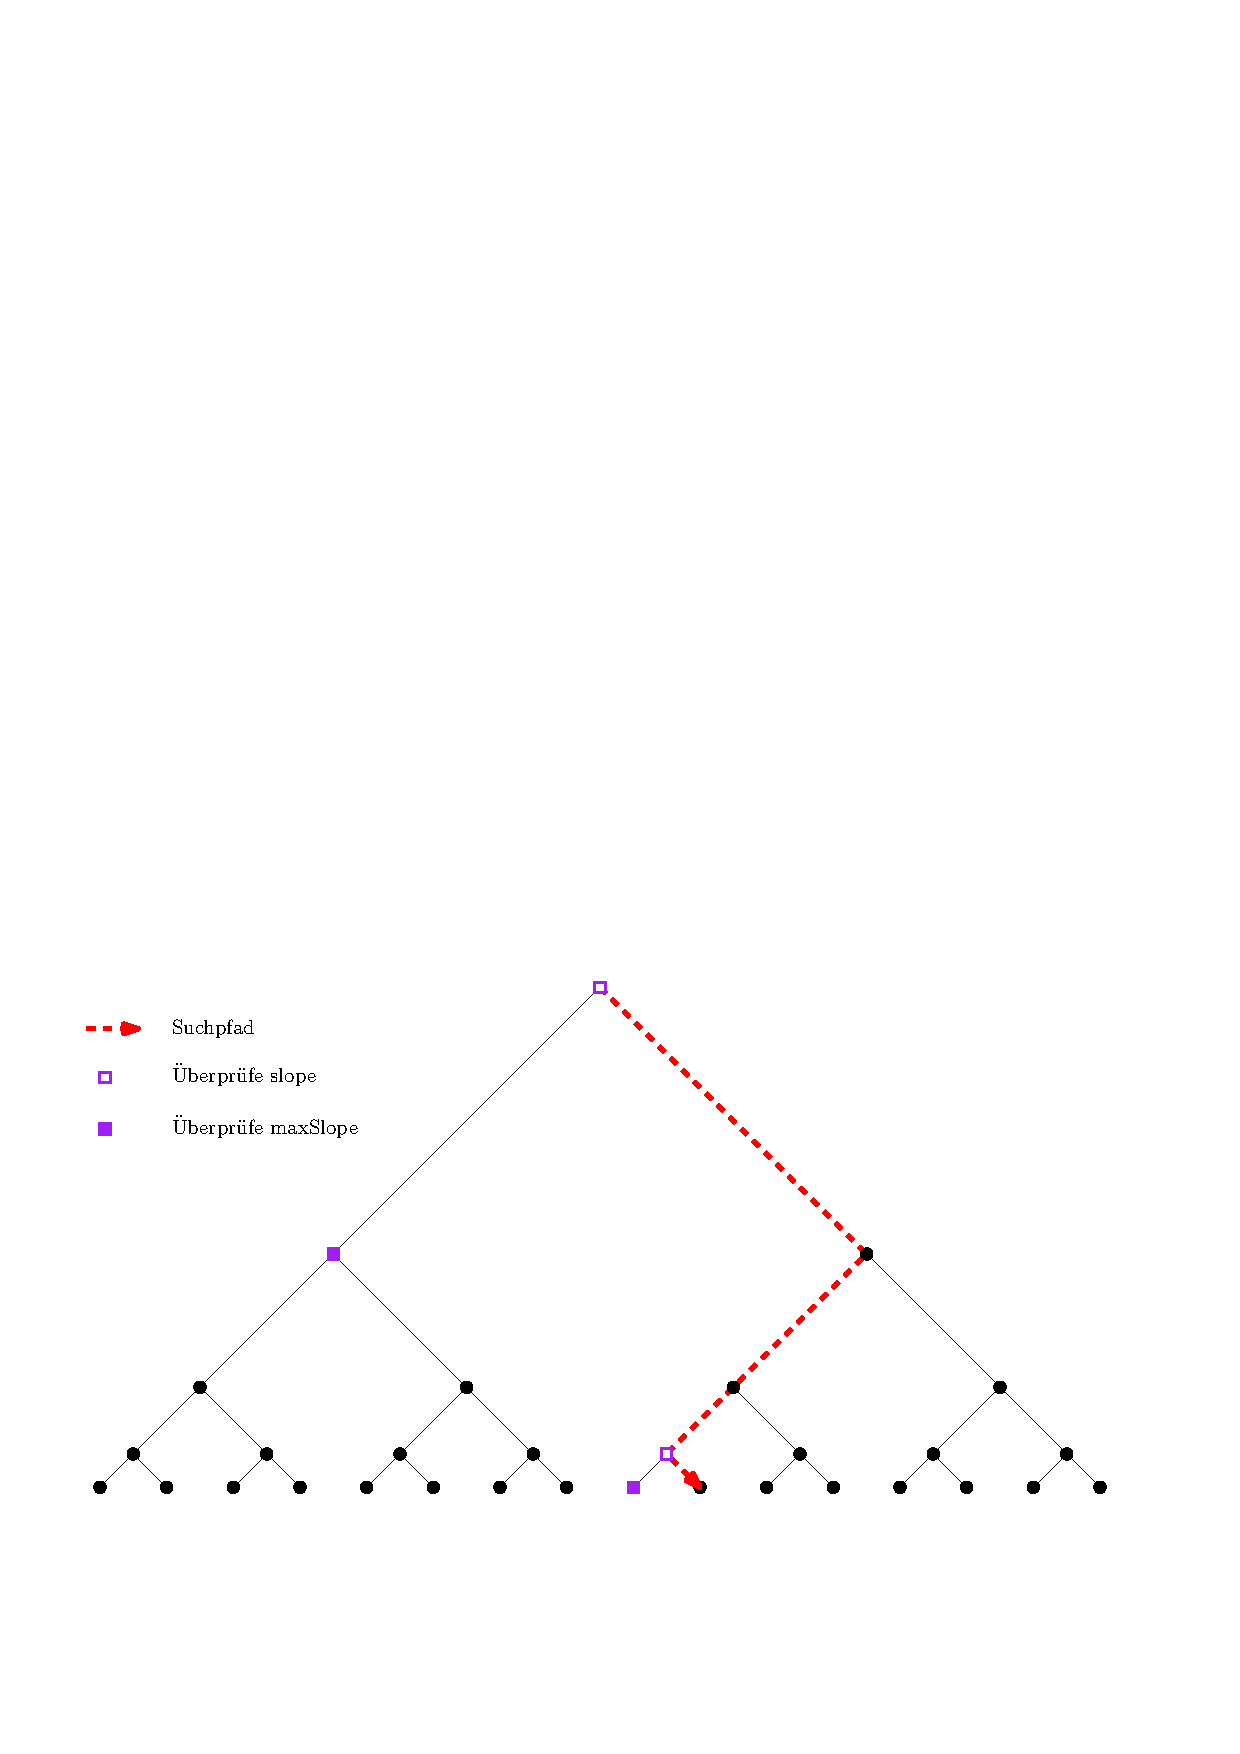
\includegraphics[width=.7\textwidth]{bilder/StatusStructure_isVisible}
    \caption[StatusStructure.isVisible(HeightedPoint pt)]{StatusStructure.isVisible(HeightedPoint pt): Die Steigung des gesuchten Punktes~pt muss mit der Steigung aller weiter links liegenden Punkte verglichen werden.}
    \label{fig:isVisible}
\end{figure}

\subsection{Speicherbedarf und Laufzeit}
\label{speicher}

Wie bereits am Ende von Kapitel \ref{sweep_adjust} erwähnt, hat die erste von uns implementierte Version des van Kreveld-Algorithmus eine 
wesentlich schlechtere Laufzeit als die des naiven Algorithmus. Durch entsprechende Tests wurde deutlich, dass bei van Krevelds Algorithmus vor allem
der Speicherbedarf eine große Rolle spielt und schnell war eines der Probleme identifiziert: die event list. Am Anfang des Programms wird die event list 
mit allen Eventtypen aller Pixel befüllt und enthält dadurch insgesamt $n \cdot n \cdot 3$ Elemente. Je größer das DEM nun ist, umso mehr Elemente 
umfasst die event list und umso mehr Speicher wird benötigt. So werden beispielsweise für ein DEM von 500x1000 Pixeln 1,5 Millionen Werte 
gleichzeitig im Speicher gehalten, was zu einer enormen Verlängerung der Laufzeit führt. 

Durch die folgenden drei Überlegungen können wir die Laufzeit des van Kreveld-Algorithmus deutlich verbessern.

\subsubsection{Verkleinern der event list}
\label{ev_klein}
Die Idee zur Verkleinerung der event list ist die folgende: Um einen enormen Speicherbedarf zu verhindern, wird die event list zu Beginn nicht mit 
allen Werten befüllt, sondern sie enthält nur die für die aktuelle Berechnung notwendigen events. Nach jeder Berechnung wird die event list dann 
aktualisiert. 

\begin{figure}[!ht]
 \centering
 \begin{BVerbatim}
  Initialisiere die Statusstruktur 
  Fülle die event list mit den auf der sweep line enthaltenen Pixeln 
  Solange die event list noch nicht leer ist 
    Do Nimm das erste event aus der Liste 
      Falls Typ == EventType.IN
	  füge Pixel in die Statusstruktur ein
      Falls Typ == EventType.OUT
	  lösche Pixel in der Statusstruktur 
      Falls Typ == EventType.CENTER
	  berechne die Sichtbarkeit des Pixels mit Hilfe der in der Statusstruktur 
	  gespeicherten Daten
      Berechne für den Pixel des events alle benachbarten Pixel 
	  Falls ein Nachbarpixel noch nicht in die event list eingefügt wurde
	       füge seine events in die event list ein
    EndDo

 \end{BVerbatim}
 \caption{Pseudocode für van Kreveld-Algorithmus mit verbesserter event list}
 \label{pseudo_krev_ev_klein}
\end{figure}

Wie aus dem Pseudocode in Abbildung \ref{pseudo_krev_ev_klein} zu entnehmen ist, wird die event list zunächst nur mit den events der Pixel befüllt,
die gerade auf der sweep line liegen -- also allen Pixeln, die rechts neben dem Standortpixel liegen und dieselbe y-Koordinate haben. Dann wird das 
erste event aus der Liste genommen und die Berechnungen durchgeführt. Bevor nun das nächste event aus der Liste genommen wird, wird die event list 
aktualisiert, d.h. wir berechnen alle Nachbarpixel des aktuellen Pixels und fügen die events dieser Pixel -- vorausgesetzt, dass diese noch nicht in 
der Liste sind -- ein. Um zu überprüfen, ob die events eines Pixels bereits in der event list sind, wird ein zweidimensionales Array mit 
den selben Abmessungen wie das DEM erstellt und dort für jeden Pixel ein boolean angelegt, dessen Wert auf \glqq true\grqq gesetzt wird, sobald die events 
des Pixels einmal in die event list eingefügt wurden.

Die Verbesserung, die sich durch diese Änderung ergibt, ist beachtlich, aber die Laufzeit liegt immer noch weit über der des naiven Algorithmus 
(siehe Kapitel \ref{exp}).

\subsubsection{Ändern der Datenstruktur der event list}

Ein weiterer Aspekt der Laufzeitoptimierung ist das Finden einer optimal(er)en Datenstruktur für die event list. Bisher haben wir die Java-interne 
Prioritätswarteschlange als Datenstruktur benutzt (PriorityQueue). Jedoch stellt sich heraus, dass eine simple ArrayList auch eine geeignete Lösung
ist und die Laufzeit nochmals verkleinern kann. Daher wird diese Änderung übernommen und entgegen des Vorschlags von van Kreveld mit einer ArrayList
weitergearbeitet. Die Verbesserung der Laufzeit ist in Kapitel \ref{exp} zu sehen.

\subsubsection{Berechnung der Winkel speichern}

Eine weitere ausschlaggebende Verbesserung ist das Ändern der Methode der Sortierung der events in die Liste. Um das event an die richtige Position 
in der event list einzufügen, wird der Winkel zum Standort berechnet und anhand dessen die Position in der Liste bestimmt. Diese Berechnung wird 
jedesmal erneut aufgerufen und führt daher zu unnötiger Rechenzeit. Um diesem Problem zuvorzukommen, wird der Wert der Winkel einmal berechnet und 
dann gespeichert (\glqq gecached\grqq). Dies führt nochmals zu einer großen Verbesserung der Laufzeit (siehe Kapitel \ref{exp}).

\subsection{Artefakte}


\newpage
\section{Experimente}
\label{exp}

\newpage
\section{Optimierungsansätze}
Die implementierten Algorithmen lassen weitere Optimierungen zu.
% - Priortätswarteschlange klein halten
Ein Optimierungsansatz, der bereits implementiert wurde, ist, die Prioritätswarteschlange der zukünfigen Ereignisse klein zu halten.
Dies wird erreicht, indem die Ereignisobjekte nach und nach erstellt und in der Warteschlange eingereiht werden,
anstatt dies gleich am Anfang des Algorithmus für alle Pixel zu tun.
Details dazu sind in Abschnitt~\ref{ev_klein} zu finden.

% - parallelisieren des Problems (Aufteilen des grids in Teile und einzeln prozessieren)
Weiterhin kann die Berechnung des Viewsheds parallelisiert werden.
Dies ist für den naiven Algorithmus besonders leicht, weil die Sichtbarkeit jedes Pixel unabhängig von allen anderen berechnet wird.
Da der naive Algorithmus mit Java-\emph{Streams} implementiert wurde und diese Parallelisierung sprachseitig unterstützen,
konnte der Algorithmus ohne Aufwand parallelisiert werden.
Bei dem Sweep-Line-Algorithmus müssen die Pixel anders aufgeteilt werden, um die Vorteile der Sweep-Line weiterhin ausnutzen zu können.
Man teilt hier die Ebene an bestimmten Winkeln auf, zum Beispiel in die vier Quadranten (das heißt an den Winkeln $0^\circ$, $90^\circ$, $180^\circ$ und $270^\circ$).
Dann überstreichen mehrere Sweep-Lines gleichzeitig die Ebene und beschleunigen so die Berechnung des Viewsheds.

% - Quadtrees
Ein weiterer Optimierungsansatz ist, den Viewshed erst nur grob zu berechnen -- also für aggregierte Pixel -- und dann graduell zu verfeinern.
Man teilt also die Ebene hierarchisch in Blöcke auf und speichert für jeden Pixelblock die minimale und maximale Höhe.
Wenn ein Pixelblock auf seiner Maximalhöhe von einem Block mit seiner Minimalhöhe verdeckt wird, kann der komplette Block als nicht sichtbar markiert werden.
Analog kann ein Pixelblock auf seiner Minimalhöhe, der von keinem Block auf seiner Maximalhöhe verdeckt wird, als sichtbar markiert werden.
Man vermeidet unter Umständen also die Berechnung der Sichtbarkeit einiger Pixel, beispielsweise wenn eine Erhebung die ganze Landschaft hinter sich verdeckt.

\newpage
\section{Fazit}

Letztendlich hat die Implementierung verschiedener Algorithmen zur Berechnung des viewsheds gezeigt, dass die Laufzeit stark von der 
Eingabe abhängt. Je kleiner die Pixelgröße des DEMs, desto höher die Laufzeit -- desto genauer aber auch die Ergebnisse. Wie jedoch in Abbildung 
\ref{dgm_erg} gezeigt, ist bei einer Pixelgröße von 1 bis 10 Metern kaum ein Unterschied mit dem bloßen Auge zu erkennen. Somit lässt sich einiges
an Rechenzeit einsparen, wenn man zunächst einen groben viewshed mit einer größeren Pixelgröße (und somit kleinere Auflösung) berechnet und dann --falls
gewünscht -- kleine Teile des DEMs genauer betrachtet. 

\bibliography{algogis}

\end{document} 